\documentclass[twoside]{book}

% Packages required by doxygen
\usepackage{fixltx2e}
\usepackage{calc}
\usepackage{doxygen}
\usepackage[export]{adjustbox} % also loads graphicx
\usepackage{graphicx}
\usepackage[utf8]{inputenc}
\usepackage{makeidx}
\usepackage{multicol}
\usepackage{multirow}
\PassOptionsToPackage{warn}{textcomp}
\usepackage{textcomp}
\usepackage[nointegrals]{wasysym}
\usepackage[table]{xcolor}

% Font selection
\usepackage[T1]{fontenc}
\usepackage[scaled=.90]{helvet}
\usepackage{courier}
\usepackage{amssymb}
\usepackage{sectsty}
\renewcommand{\familydefault}{\sfdefault}
\allsectionsfont{%
  \fontseries{bc}\selectfont%
  \color{darkgray}%
}
\renewcommand{\DoxyLabelFont}{%
  \fontseries{bc}\selectfont%
  \color{darkgray}%
}
\newcommand{\+}{\discretionary{\mbox{\scriptsize$\hookleftarrow$}}{}{}}

% Page & text layout
\usepackage{geometry}
\geometry{%
  a4paper,%
  top=2.5cm,%
  bottom=2.5cm,%
  left=2.5cm,%
  right=2.5cm%
}
\tolerance=750
\hfuzz=15pt
\hbadness=750
\setlength{\emergencystretch}{15pt}
\setlength{\parindent}{0cm}
\setlength{\parskip}{3ex plus 2ex minus 2ex}
\makeatletter
\renewcommand{\paragraph}{%
  \@startsection{paragraph}{4}{0ex}{-1.0ex}{1.0ex}{%
    \normalfont\normalsize\bfseries\SS@parafont%
  }%
}
\renewcommand{\subparagraph}{%
  \@startsection{subparagraph}{5}{0ex}{-1.0ex}{1.0ex}{%
    \normalfont\normalsize\bfseries\SS@subparafont%
  }%
}
\makeatother

% Headers & footers
\usepackage{fancyhdr}
\pagestyle{fancyplain}
\fancyhead[LE]{\fancyplain{}{\bfseries\thepage}}
\fancyhead[CE]{\fancyplain{}{}}
\fancyhead[RE]{\fancyplain{}{\bfseries\leftmark}}
\fancyhead[LO]{\fancyplain{}{\bfseries\rightmark}}
\fancyhead[CO]{\fancyplain{}{}}
\fancyhead[RO]{\fancyplain{}{\bfseries\thepage}}
\fancyfoot[LE]{\fancyplain{}{}}
\fancyfoot[CE]{\fancyplain{}{}}
\fancyfoot[RE]{\fancyplain{}{\bfseries\scriptsize Generated by Doxygen }}
\fancyfoot[LO]{\fancyplain{}{\bfseries\scriptsize Generated by Doxygen }}
\fancyfoot[CO]{\fancyplain{}{}}
\fancyfoot[RO]{\fancyplain{}{}}
\renewcommand{\footrulewidth}{0.4pt}
\renewcommand{\chaptermark}[1]{%
  \markboth{#1}{}%
}
\renewcommand{\sectionmark}[1]{%
  \markright{\thesection\ #1}%
}

% Indices & bibliography
\usepackage{natbib}
\usepackage[titles]{tocloft}
\setcounter{tocdepth}{3}
\setcounter{secnumdepth}{5}
\makeindex

% Hyperlinks (required, but should be loaded last)
\usepackage{ifpdf}
\ifpdf
  \usepackage[pdftex,pagebackref=true]{hyperref}
\else
  \usepackage[ps2pdf,pagebackref=true]{hyperref}
\fi
\hypersetup{%
  colorlinks=true,%
  linkcolor=blue,%
  citecolor=blue,%
  unicode%
}

% Custom commands
\newcommand{\clearemptydoublepage}{%
  \newpage{\pagestyle{empty}\cleardoublepage}%
}

\usepackage{caption}
\captionsetup{labelsep=space,justification=centering,font={bf},singlelinecheck=off,skip=4pt,position=top}

%===== C O N T E N T S =====

\begin{document}

% Titlepage & ToC
\hypersetup{pageanchor=false,
             bookmarksnumbered=true,
             pdfencoding=unicode
            }
\pagenumbering{roman}
\begin{titlepage}
\vspace*{7cm}
\begin{center}%
{\Large Human Obstacle Detector }\\
\vspace*{1cm}
{\large Generated by Doxygen 1.8.11}\\
\end{center}
\end{titlepage}
\clearemptydoublepage
\tableofcontents
\clearemptydoublepage
\pagenumbering{arabic}
\hypersetup{pageanchor=true}

%--- Begin generated contents ---
\chapter{Class Index}
\section{Class List}
Here are the classes, structs, unions and interfaces with brief descriptions\+:\begin{DoxyCompactList}
\item\contentsline{section}{\hyperlink{classData}{Data} }{\pageref{classData}}{}
\item\contentsline{section}{\hyperlink{classDetection}{Detection} }{\pageref{classDetection}}{}
\item\contentsline{section}{\hyperlink{classLocator}{Locator} }{\pageref{classLocator}}{}
\item\contentsline{section}{\hyperlink{classProgramOptions}{Program\+Options} }{\pageref{classProgramOptions}}{}
\end{DoxyCompactList}

\chapter{File Index}
\section{File List}
Here is a list of all documented files with brief descriptions\+:\begin{DoxyCompactList}
\item\contentsline{section}{app/\hyperlink{data_8cpp}{data.\+cpp} }{\pageref{data_8cpp}}{}
\item\contentsline{section}{app/\hyperlink{detection_8cpp}{detection.\+cpp} }{\pageref{detection_8cpp}}{}
\item\contentsline{section}{app/\hyperlink{locator_8cpp}{locator.\+cpp} \\*End result of class is to return the position of the object desired. Class will receive dimensions and starting pixel position of a bounding box, and from there determine the world coordinate position depending on the camera. Here we assume the intrinsic and extrinsic parameters of the camera }{\pageref{locator_8cpp}}{}
\item\contentsline{section}{app/\hyperlink{program__options_8cpp}{program\+\_\+options.\+cpp} \\*This class allows for command line arguments for file paths }{\pageref{program__options_8cpp}}{}
\item\contentsline{section}{include/\hyperlink{data_8hpp}{data.\+hpp} \\*Loads data files (images) }{\pageref{data_8hpp}}{}
\item\contentsline{section}{include/\hyperlink{detection_8hpp}{detection.\+hpp} }{\pageref{detection_8hpp}}{}
\item\contentsline{section}{include/\hyperlink{locator_8hpp}{locator.\+hpp} \\*End result of class is to return the position of the object desired. Class will receive dimensions and starting pixel position of a bounding box, and from there determine the world coordinate position depending on the camera. Here we assume the intrinsic and extrinsic parameters of the camera }{\pageref{locator_8hpp}}{}
\item\contentsline{section}{include/\hyperlink{program__options_8hpp}{program\+\_\+options.\+hpp} \\*Class allows for command line arguments for setting path }{\pageref{program__options_8hpp}}{}
\item\contentsline{section}{test/\hyperlink{data__test_8cpp}{data\+\_\+test.\+cpp} \\*Unit Test for \hyperlink{classData}{Data} Class }{\pageref{data__test_8cpp}}{}
\item\contentsline{section}{test/\hyperlink{detection__test_8cpp}{detection\+\_\+test.\+cpp} \\*Unit Test for \hyperlink{classDetection}{Detection} Class }{\pageref{detection__test_8cpp}}{}
\item\contentsline{section}{test/\hyperlink{locator__test_8cpp}{locator\+\_\+test.\+cpp} \\*Unit Tests for \hyperlink{classLocator}{Locator} }{\pageref{locator__test_8cpp}}{}
\item\contentsline{section}{test/\hyperlink{program__options__test_8cpp}{program\+\_\+options\+\_\+test.\+cpp} \\*Unit Test for \hyperlink{classProgramOptions}{Program\+Options} Class }{\pageref{program__options__test_8cpp}}{}
\end{DoxyCompactList}

\chapter{Class Documentation}
\hypertarget{classData}{}\section{Data Class Reference}
\label{classData}\index{Data@{Data}}


{\ttfamily \#include $<$data.\+hpp$>$}

\subsection*{Static Public Member Functions}
\begin{DoxyCompactItemize}
\item 
static cv\+::\+Mat \hyperlink{classData_a998ab1e595e2f02aa0a9af2ff68274ab}{load\+Image} (const std\+::string \&file\+Path)
\item 
static std\+::vector$<$ cv\+::\+Mat $>$ \hyperlink{classData_af7e7f6fe68b1f70ced7bae1d379dc59a}{load\+Images} (const std\+::string \&files\+Dir)
\end{DoxyCompactItemize}


\subsection{Detailed Description}
Handles image data loading. 

\subsection{Member Function Documentation}
\index{Data@{Data}!load\+Image@{load\+Image}}
\index{load\+Image@{load\+Image}!Data@{Data}}
\subsubsection[{\texorpdfstring{load\+Image(const std\+::string \&file\+Path)}{loadImage(const std::string &filePath)}}]{\setlength{\rightskip}{0pt plus 5cm}cv\+::\+Mat Data\+::load\+Image (
\begin{DoxyParamCaption}
\item[{const std\+::string \&}]{file\+Path}
\end{DoxyParamCaption}
)\hspace{0.3cm}{\ttfamily [static]}}\hypertarget{classData_a998ab1e595e2f02aa0a9af2ff68274ab}{}\label{classData_a998ab1e595e2f02aa0a9af2ff68274ab}
Load an image. 
\begin{DoxyParams}{Parameters}
{\em file\+Path} & path to image \\
\hline
\end{DoxyParams}
\begin{DoxyReturn}{Returns}
image 
\end{DoxyReturn}
\index{Data@{Data}!load\+Images@{load\+Images}}
\index{load\+Images@{load\+Images}!Data@{Data}}
\subsubsection[{\texorpdfstring{load\+Images(const std\+::string \&files\+Dir)}{loadImages(const std::string &filesDir)}}]{\setlength{\rightskip}{0pt plus 5cm}std\+::vector$<$ cv\+::\+Mat $>$ Data\+::load\+Images (
\begin{DoxyParamCaption}
\item[{const std\+::string \&}]{files\+Dir}
\end{DoxyParamCaption}
)\hspace{0.3cm}{\ttfamily [static]}}\hypertarget{classData_af7e7f6fe68b1f70ced7bae1d379dc59a}{}\label{classData_af7e7f6fe68b1f70ced7bae1d379dc59a}
Load all images in a directory. 
\begin{DoxyParams}{Parameters}
{\em files\+Path} & directory containing images \\
\hline
\end{DoxyParams}
\begin{DoxyReturn}{Returns}
vector of images 
\end{DoxyReturn}


The documentation for this class was generated from the following files\+:\begin{DoxyCompactItemize}
\item 
include/\hyperlink{data_8hpp}{data.\+hpp}\item 
app/\hyperlink{data_8cpp}{data.\+cpp}\end{DoxyCompactItemize}

\hypertarget{classDetection}{}\section{Detection Class Reference}
\label{classDetection}\index{Detection@{Detection}}


{\ttfamily \#include $<$detection.\+hpp$>$}

\subsection*{Public Member Functions}
\begin{DoxyCompactItemize}
\item 
\hyperlink{classDetection_a86e6ebf5a660a29e78ee7a7f08292260}{Detection} ()
\item 
std\+::vector$<$ cv\+::\+Rect $>$ \hyperlink{classDetection_a039afb9f14939240b1ec7dd00c04fbfe}{detect} (const cv\+::\+Mat \&image)
\end{DoxyCompactItemize}


\subsection{Detailed Description}
Performs Histogram of Gradients detection of humans in images using Support Vector Machines. 

\subsection{Constructor \& Destructor Documentation}
\index{Detection@{Detection}!Detection@{Detection}}
\index{Detection@{Detection}!Detection@{Detection}}
\subsubsection[{\texorpdfstring{Detection()}{Detection()}}]{\setlength{\rightskip}{0pt plus 5cm}Detection\+::\+Detection (
\begin{DoxyParamCaption}
{}
\end{DoxyParamCaption}
)}\hypertarget{classDetection_a86e6ebf5a660a29e78ee7a7f08292260}{}\label{classDetection_a86e6ebf5a660a29e78ee7a7f08292260}
Initializes the H\+OG descriptor. 

\subsection{Member Function Documentation}
\index{Detection@{Detection}!detect@{detect}}
\index{detect@{detect}!Detection@{Detection}}
\subsubsection[{\texorpdfstring{detect(const cv\+::\+Mat \&image)}{detect(const cv::Mat &image)}}]{\setlength{\rightskip}{0pt plus 5cm}std\+::vector$<$ cv\+::\+Rect $>$ Detection\+::detect (
\begin{DoxyParamCaption}
\item[{const cv\+::\+Mat \&}]{image}
\end{DoxyParamCaption}
)}\hypertarget{classDetection_a039afb9f14939240b1ec7dd00c04fbfe}{}\label{classDetection_a039afb9f14939240b1ec7dd00c04fbfe}
Detects humans in images using H\+OG and the Open\+CV S\+VM default people detector. 
\begin{DoxyParams}{Parameters}
{\em image} & \\
\hline
\end{DoxyParams}
\begin{DoxyReturn}{Returns}

\end{DoxyReturn}


The documentation for this class was generated from the following files\+:\begin{DoxyCompactItemize}
\item 
include/\hyperlink{detection_8hpp}{detection.\+hpp}\item 
app/\hyperlink{detection_8cpp}{detection.\+cpp}\end{DoxyCompactItemize}

\hypertarget{classLocator}{}\section{Locator Class Reference}
\label{classLocator}\index{Locator@{Locator}}
\subsection*{Public Member Functions}
\begin{DoxyCompactItemize}
\item 
\hyperlink{classLocator_a309b4d4180297ebe1a15c3ddff22bb0a}{Locator} ()
\begin{DoxyCompactList}\small\item\em Default constructor for locator class. This is for demo purposes. The non-\/default constructor should be used to set camera parameters in cv\+::\+Mat format. \end{DoxyCompactList}\item 
\hyperlink{classLocator_a2a33d04a9b0355c7a60f2c5e7114689a}{Locator} (cv\+::\+Mat rotationM, cv\+::\+Mat translation\+Vec, cv\+::\+Mat intrinsicM)
\begin{DoxyCompactList}\small\item\em Constructor to set camera parameters. All parameters should be in matrix form (cv\+::\+Mat). \end{DoxyCompactList}\item 
void \hyperlink{classLocator_a2a1903c4adab7ebecd1f4790a135a39a}{set\+Pixel\+Data} (cv\+::\+Rect \&pixel\+Data)
\begin{DoxyCompactList}\small\item\em Receives pixel data as type cv\+::\+Rect, and sets it to the private attribute pixel\+Point. It later uses the private method pixel\+Vector() to extract important information of data given, and creates a vector of type cv\+::\+Mat. \end{DoxyCompactList}\item 
cv\+::\+Rect \hyperlink{classLocator_abe66e0f8d5c7786be8c2154bfab43fc1}{get\+Pixel\+Data} ()
\begin{DoxyCompactList}\small\item\em Gets pixel\+Data. \end{DoxyCompactList}\item 
void \hyperlink{classLocator_a9c7db372b262aac0f02c774ac3753e10}{world\+Pos} ()
\begin{DoxyCompactList}\small\item\em Calculations to obtain Real World Coordinates. Highly important to detect distance of object. \end{DoxyCompactList}\item 
void \hyperlink{classLocator_ae702d1254f48d0b37d0e98612fde768d}{print\+Positions} ()
\begin{DoxyCompactList}\small\item\em Prints the Real World Coordinates. \end{DoxyCompactList}\item 
cv\+::\+Mat \hyperlink{classLocator_a0ddf0eb54e7af896ac04654602d2459d}{get\+Rotation\+Matrix} ()
\begin{DoxyCompactList}\small\item\em Getter method to return rotation matrix. Mostly used for unit testing. \end{DoxyCompactList}\item 
cv\+::\+Mat \hyperlink{classLocator_a9a34468f1f815a132ab3dbf62b883fb7}{get\+Translation\+Vector} ()
\begin{DoxyCompactList}\small\item\em Getter method to return translation vector. Mostly used for unit testing. \end{DoxyCompactList}\item 
cv\+::\+Mat \hyperlink{classLocator_a551e2fe1ea1d84838651d2a4716707b5}{get\+Instrinsic\+Matrix} ()
\begin{DoxyCompactList}\small\item\em Getter method to return intrinsic matrix. Mostly used for unit testing. \end{DoxyCompactList}\end{DoxyCompactItemize}
\subsection*{Public Attributes}
\begin{DoxyCompactItemize}
\item 
cv\+::\+Mat \hyperlink{classLocator_ac9f5a8f6aa5dd57776947961ca49098a}{world\+Coord}\hypertarget{classLocator_ac9f5a8f6aa5dd57776947961ca49098a}{}\label{classLocator_ac9f5a8f6aa5dd57776947961ca49098a}

\begin{DoxyCompactList}\small\item\em World Coordinates in cv\+::\+Mat datatype. \end{DoxyCompactList}\end{DoxyCompactItemize}


\subsection{Constructor \& Destructor Documentation}
\index{Locator@{Locator}!Locator@{Locator}}
\index{Locator@{Locator}!Locator@{Locator}}
\subsubsection[{\texorpdfstring{Locator()}{Locator()}}]{\setlength{\rightskip}{0pt plus 5cm}Locator\+::\+Locator (
\begin{DoxyParamCaption}
{}
\end{DoxyParamCaption}
)}\hypertarget{classLocator_a309b4d4180297ebe1a15c3ddff22bb0a}{}\label{classLocator_a309b4d4180297ebe1a15c3ddff22bb0a}


Default constructor for locator class. This is for demo purposes. The non-\/default constructor should be used to set camera parameters in cv\+::\+Mat format. 


\begin{DoxyParams}{Parameters}
{\em none} & \\
\hline
\end{DoxyParams}
\begin{DoxyReturn}{Returns}
none 
\end{DoxyReturn}
rotation matrix is conformed of \mbox{[}r1 r2 translation\mbox{]}. r3 isn\textquotesingle{}t necessary because it is a redundant cross product of the first 2 columns \index{Locator@{Locator}!Locator@{Locator}}
\index{Locator@{Locator}!Locator@{Locator}}
\subsubsection[{\texorpdfstring{Locator(cv\+::\+Mat rotation\+M, cv\+::\+Mat translation\+Vec, cv\+::\+Mat intrinsic\+M)}{Locator(cv::Mat rotationM, cv::Mat translationVec, cv::Mat intrinsicM)}}]{\setlength{\rightskip}{0pt plus 5cm}Locator\+::\+Locator (
\begin{DoxyParamCaption}
\item[{cv\+::\+Mat}]{rotationM, }
\item[{cv\+::\+Mat}]{translation\+Vec, }
\item[{cv\+::\+Mat}]{intrinsicM}
\end{DoxyParamCaption}
)}\hypertarget{classLocator_a2a33d04a9b0355c7a60f2c5e7114689a}{}\label{classLocator_a2a33d04a9b0355c7a60f2c5e7114689a}


Constructor to set camera parameters. All parameters should be in matrix form (cv\+::\+Mat). 


\begin{DoxyParams}{Parameters}
{\em rotationM,translation\+Vec,intrinsicM} & These are the parameters in which to get accurate 3D position. \\
\hline
\end{DoxyParams}
\begin{DoxyReturn}{Returns}
none 
\end{DoxyReturn}
Check size of matrix 

\subsection{Member Function Documentation}
\index{Locator@{Locator}!get\+Instrinsic\+Matrix@{get\+Instrinsic\+Matrix}}
\index{get\+Instrinsic\+Matrix@{get\+Instrinsic\+Matrix}!Locator@{Locator}}
\subsubsection[{\texorpdfstring{get\+Instrinsic\+Matrix()}{getInstrinsicMatrix()}}]{\setlength{\rightskip}{0pt plus 5cm}cv\+::\+Mat Locator\+::get\+Instrinsic\+Matrix (
\begin{DoxyParamCaption}
{}
\end{DoxyParamCaption}
)}\hypertarget{classLocator_a551e2fe1ea1d84838651d2a4716707b5}{}\label{classLocator_a551e2fe1ea1d84838651d2a4716707b5}


Getter method to return intrinsic matrix. Mostly used for unit testing. 


\begin{DoxyParams}{Parameters}
{\em none} & \\
\hline
\end{DoxyParams}
\begin{DoxyReturn}{Returns}
\+\_\+intrinsicM Intrinsic Matrix as cv\+::\+Mat 
\end{DoxyReturn}
\index{Locator@{Locator}!get\+Pixel\+Data@{get\+Pixel\+Data}}
\index{get\+Pixel\+Data@{get\+Pixel\+Data}!Locator@{Locator}}
\subsubsection[{\texorpdfstring{get\+Pixel\+Data()}{getPixelData()}}]{\setlength{\rightskip}{0pt plus 5cm}cv\+::\+Rect Locator\+::get\+Pixel\+Data (
\begin{DoxyParamCaption}
{}
\end{DoxyParamCaption}
)}\hypertarget{classLocator_abe66e0f8d5c7786be8c2154bfab43fc1}{}\label{classLocator_abe66e0f8d5c7786be8c2154bfab43fc1}


Gets pixel\+Data. 


\begin{DoxyParams}{Parameters}
{\em none} & \\
\hline
\end{DoxyParams}
\begin{DoxyReturn}{Returns}
none 
\end{DoxyReturn}
\index{Locator@{Locator}!get\+Rotation\+Matrix@{get\+Rotation\+Matrix}}
\index{get\+Rotation\+Matrix@{get\+Rotation\+Matrix}!Locator@{Locator}}
\subsubsection[{\texorpdfstring{get\+Rotation\+Matrix()}{getRotationMatrix()}}]{\setlength{\rightskip}{0pt plus 5cm}cv\+::\+Mat Locator\+::get\+Rotation\+Matrix (
\begin{DoxyParamCaption}
{}
\end{DoxyParamCaption}
)}\hypertarget{classLocator_a0ddf0eb54e7af896ac04654602d2459d}{}\label{classLocator_a0ddf0eb54e7af896ac04654602d2459d}


Getter method to return rotation matrix. Mostly used for unit testing. 


\begin{DoxyParams}{Parameters}
{\em none} & \\
\hline
\end{DoxyParams}
\begin{DoxyReturn}{Returns}
\+\_\+rotationM Rotation matrix as cv\+::\+Mat 
\end{DoxyReturn}
\index{Locator@{Locator}!get\+Translation\+Vector@{get\+Translation\+Vector}}
\index{get\+Translation\+Vector@{get\+Translation\+Vector}!Locator@{Locator}}
\subsubsection[{\texorpdfstring{get\+Translation\+Vector()}{getTranslationVector()}}]{\setlength{\rightskip}{0pt plus 5cm}cv\+::\+Mat Locator\+::get\+Translation\+Vector (
\begin{DoxyParamCaption}
{}
\end{DoxyParamCaption}
)}\hypertarget{classLocator_a9a34468f1f815a132ab3dbf62b883fb7}{}\label{classLocator_a9a34468f1f815a132ab3dbf62b883fb7}


Getter method to return translation vector. Mostly used for unit testing. 


\begin{DoxyParams}{Parameters}
{\em none} & \\
\hline
\end{DoxyParams}
\begin{DoxyReturn}{Returns}
\+\_\+trans\+Vec Trasnlation vector as cv\+::\+Mat 
\end{DoxyReturn}
\index{Locator@{Locator}!print\+Positions@{print\+Positions}}
\index{print\+Positions@{print\+Positions}!Locator@{Locator}}
\subsubsection[{\texorpdfstring{print\+Positions()}{printPositions()}}]{\setlength{\rightskip}{0pt plus 5cm}void Locator\+::print\+Positions (
\begin{DoxyParamCaption}
{}
\end{DoxyParamCaption}
)}\hypertarget{classLocator_ae702d1254f48d0b37d0e98612fde768d}{}\label{classLocator_ae702d1254f48d0b37d0e98612fde768d}


Prints the Real World Coordinates. 


\begin{DoxyParams}{Parameters}
{\em none} & \\
\hline
\end{DoxyParams}
\begin{DoxyReturn}{Returns}
none 
\end{DoxyReturn}
Prints position of object detected (human in this case). \index{Locator@{Locator}!set\+Pixel\+Data@{set\+Pixel\+Data}}
\index{set\+Pixel\+Data@{set\+Pixel\+Data}!Locator@{Locator}}
\subsubsection[{\texorpdfstring{set\+Pixel\+Data(cv\+::\+Rect \&pixel\+Data)}{setPixelData(cv::Rect &pixelData)}}]{\setlength{\rightskip}{0pt plus 5cm}void Locator\+::set\+Pixel\+Data (
\begin{DoxyParamCaption}
\item[{cv\+::\+Rect \&}]{pixel\+Data}
\end{DoxyParamCaption}
)}\hypertarget{classLocator_a2a1903c4adab7ebecd1f4790a135a39a}{}\label{classLocator_a2a1903c4adab7ebecd1f4790a135a39a}


Receives pixel data as type cv\+::\+Rect, and sets it to the private attribute pixel\+Point. It later uses the private method pixel\+Vector() to extract important information of data given, and creates a vector of type cv\+::\+Mat. 


\begin{DoxyParams}{Parameters}
{\em pixel\+Data} & pixel data which is given as bounding box information \\
\hline
\end{DoxyParams}
\begin{DoxyReturn}{Returns}
none 
\end{DoxyReturn}
Sets pixel\+Data to attribute pixel\+Point \index{Locator@{Locator}!world\+Pos@{world\+Pos}}
\index{world\+Pos@{world\+Pos}!Locator@{Locator}}
\subsubsection[{\texorpdfstring{world\+Pos()}{worldPos()}}]{\setlength{\rightskip}{0pt plus 5cm}void Locator\+::world\+Pos (
\begin{DoxyParamCaption}
{}
\end{DoxyParamCaption}
)}\hypertarget{classLocator_a9c7db372b262aac0f02c774ac3753e10}{}\label{classLocator_a9c7db372b262aac0f02c774ac3753e10}


Calculations to obtain Real World Coordinates. Highly important to detect distance of object. 


\begin{DoxyParams}{Parameters}
{\em none} & \\
\hline
\end{DoxyParams}
\begin{DoxyReturn}{Returns}
none 
\end{DoxyReturn}
Calculates real world coordinate with intrinsic and extrinsic camera parameters.

world\+Coord = (((pixel\+Coord $\ast$ \+\_\+intrinsic\+M.\+inv()) -\/ \+\_\+trans\+Vec ) $\ast$ \+\_\+rotation\+M.\+inv()) / 1000; 

The documentation for this class was generated from the following files\+:\begin{DoxyCompactItemize}
\item 
include/\hyperlink{locator_8hpp}{locator.\+hpp}\item 
app/\hyperlink{locator_8cpp}{locator.\+cpp}\end{DoxyCompactItemize}

\hypertarget{classProgramOptions}{}\section{Program\+Options Class Reference}
\label{classProgramOptions}\index{Program\+Options@{Program\+Options}}


{\ttfamily \#include $<$program\+\_\+options.\+hpp$>$}

\subsection*{Public Member Functions}
\begin{DoxyCompactItemize}
\item 
\hyperlink{classProgramOptions_af4d748ab66175b1a0c67d38f96403eff}{Program\+Options} ()
\item 
void \hyperlink{classProgramOptions_ab2603a54fd83c450cf81d074f061d0ee}{parse} (int argc, const char $\ast$argv\mbox{[}$\,$\mbox{]})
\item 
std\+::string \hyperlink{classProgramOptions_a18eb214deb1a7196986dc0269bbdad4c}{get\+Value} (const std\+::string \&option\+Name)
\end{DoxyCompactItemize}


\subsection{Detailed Description}
Defines available program options and retrieves option values. 

\subsection{Constructor \& Destructor Documentation}
\index{Program\+Options@{Program\+Options}!Program\+Options@{Program\+Options}}
\index{Program\+Options@{Program\+Options}!Program\+Options@{Program\+Options}}
\subsubsection[{\texorpdfstring{Program\+Options()}{ProgramOptions()}}]{\setlength{\rightskip}{0pt plus 5cm}Program\+Options\+::\+Program\+Options (
\begin{DoxyParamCaption}
{}
\end{DoxyParamCaption}
)}\hypertarget{classProgramOptions_af4d748ab66175b1a0c67d38f96403eff}{}\label{classProgramOptions_af4d748ab66175b1a0c67d38f96403eff}
add program options 

\subsection{Member Function Documentation}
\index{Program\+Options@{Program\+Options}!get\+Value@{get\+Value}}
\index{get\+Value@{get\+Value}!Program\+Options@{Program\+Options}}
\subsubsection[{\texorpdfstring{get\+Value(const std\+::string \&option\+Name)}{getValue(const std::string &optionName)}}]{\setlength{\rightskip}{0pt plus 5cm}std\+::string Program\+Options\+::get\+Value (
\begin{DoxyParamCaption}
\item[{const std\+::string \&}]{option\+Name}
\end{DoxyParamCaption}
)}\hypertarget{classProgramOptions_a18eb214deb1a7196986dc0269bbdad4c}{}\label{classProgramOptions_a18eb214deb1a7196986dc0269bbdad4c}
Gets the value for an options 
\begin{DoxyParams}{Parameters}
{\em option\+Name} & the name of the option \\
\hline
\end{DoxyParams}
\begin{DoxyReturn}{Returns}
the option value 
\end{DoxyReturn}
if the option is not provided, throw an exception and print the options

get the option value \index{Program\+Options@{Program\+Options}!parse@{parse}}
\index{parse@{parse}!Program\+Options@{Program\+Options}}
\subsubsection[{\texorpdfstring{parse(int argc, const char $\ast$argv[])}{parse(int argc, const char *argv[])}}]{\setlength{\rightskip}{0pt plus 5cm}void Program\+Options\+::parse (
\begin{DoxyParamCaption}
\item[{int}]{argc, }
\item[{const char $\ast$}]{argv\mbox{[}$\,$\mbox{]}}
\end{DoxyParamCaption}
)}\hypertarget{classProgramOptions_ab2603a54fd83c450cf81d074f061d0ee}{}\label{classProgramOptions_ab2603a54fd83c450cf81d074f061d0ee}
Parse command line arguments as options. 
\begin{DoxyParams}{Parameters}
{\em argc} & the number of arguments \\
\hline
{\em argv} & the list of arguments \\
\hline
\end{DoxyParams}
get and store the parsed options

if no options provided, stop program and print options

if help option provided, stop program and print options 

The documentation for this class was generated from the following files\+:\begin{DoxyCompactItemize}
\item 
include/\hyperlink{program__options_8hpp}{program\+\_\+options.\+hpp}\item 
app/\hyperlink{program__options_8cpp}{program\+\_\+options.\+cpp}\end{DoxyCompactItemize}

\chapter{File Documentation}
\hypertarget{data_8cpp}{}\section{app/data.cpp File Reference}
\label{data_8cpp}\index{app/data.\+cpp@{app/data.\+cpp}}
{\ttfamily \#include \char`\"{}data.\+hpp\char`\"{}}\\*
{\ttfamily \#include $<$string$>$}\\*
{\ttfamily \#include $<$vector$>$}\\*
Include dependency graph for data.\+cpp\+:
\nopagebreak
\begin{figure}[H]
\begin{center}
\leavevmode
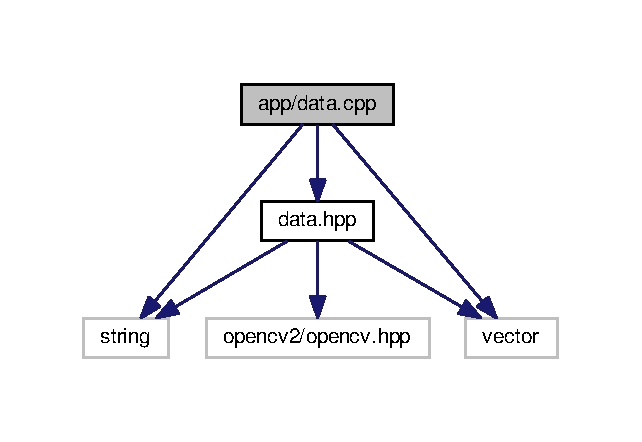
\includegraphics[width=308pt]{data_8cpp__incl}
\end{center}
\end{figure}


\subsection{Detailed Description}
\begin{DoxyAuthor}{Author}
Pablo Sanhueza 

Ryan Cunningham 

Andre Gomes 
\end{DoxyAuthor}
\begin{DoxyCopyright}{Copyright}
2019 Distributed under the B\+SD License (license terms found in L\+I\+C\+E\+N\+SE or at \href{https://www.freebsd.org/copyright/freebsd-license.html}{\tt https\+://www.\+freebsd.\+org/copyright/freebsd-\/license.\+html}) 
\end{DoxyCopyright}

\hypertarget{detection_8cpp}{}\section{app/detection.cpp File Reference}
\label{detection_8cpp}\index{app/detection.\+cpp@{app/detection.\+cpp}}
{\ttfamily \#include \char`\"{}detection.\+hpp\char`\"{}}\\*
{\ttfamily \#include $<$opencv2/opencv.\+hpp$>$}\\*
{\ttfamily \#include $<$vector$>$}\\*
Include dependency graph for detection.\+cpp\+:
\nopagebreak
\begin{figure}[H]
\begin{center}
\leavevmode
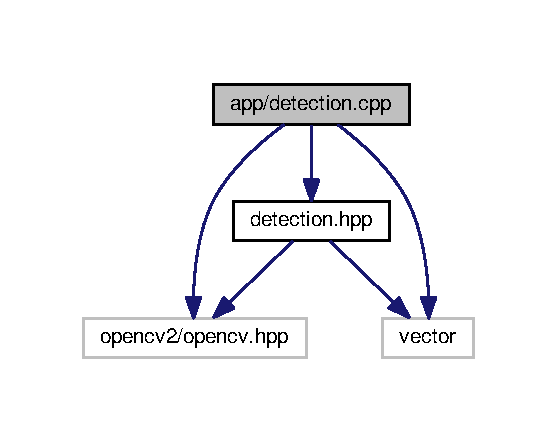
\includegraphics[width=268pt]{detection_8cpp__incl}
\end{center}
\end{figure}


\subsection{Detailed Description}
\begin{DoxyAuthor}{Author}

\end{DoxyAuthor}
\begin{DoxyCopyright}{Copyright}
2019 Distributed under the B\+SD License (license terms found in L\+I\+C\+E\+N\+SE or at \href{https://www.freebsd.org/copyright/freebsd-license.html}{\tt https\+://www.\+freebsd.\+org/copyright/freebsd-\/license.\+html}) 
\end{DoxyCopyright}

\hypertarget{locator_8cpp}{}\section{app/locator.cpp File Reference}
\label{locator_8cpp}\index{app/locator.\+cpp@{app/locator.\+cpp}}


End result of class is to return the position of the object desired. Class will receive dimensions and starting pixel position of a bounding box, and from there determine the world coordinate position depending on the camera. Here we assume the intrinsic and extrinsic parameters of the camera.  


{\ttfamily \#include $<$iostream$>$}\\*
{\ttfamily \#include $<$opencv2/opencv.\+hpp$>$}\\*
{\ttfamily \#include $<$string$>$}\\*
{\ttfamily \#include $<$vector$>$}\\*
{\ttfamily \#include \char`\"{}locator.\+hpp\char`\"{}}\\*
Include dependency graph for locator.\+cpp\+:
\nopagebreak
\begin{figure}[H]
\begin{center}
\leavevmode
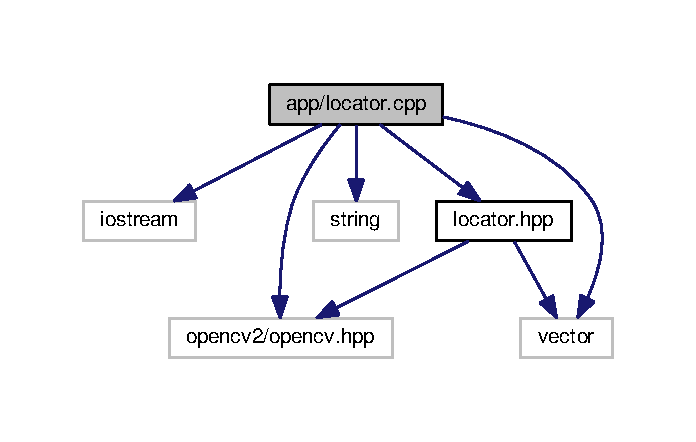
\includegraphics[width=334pt]{locator_8cpp__incl}
\end{center}
\end{figure}


\subsection{Detailed Description}
End result of class is to return the position of the object desired. Class will receive dimensions and starting pixel position of a bounding box, and from there determine the world coordinate position depending on the camera. Here we assume the intrinsic and extrinsic parameters of the camera. 

\begin{DoxyAuthor}{Author}
Pablo Sanhueza 

Andre Gomes 

Ryan Cunningham
\end{DoxyAuthor}
\begin{DoxyCopyright}{Copyright}
2019 Pablo Sanhueza, Andre Gomes, Ryan Cunningham 
\end{DoxyCopyright}

\hypertarget{program__options_8cpp}{}\section{app/program\+\_\+options.cpp File Reference}
\label{program__options_8cpp}\index{app/program\+\_\+options.\+cpp@{app/program\+\_\+options.\+cpp}}


This class allows for command line arguments for file paths.  


{\ttfamily \#include \char`\"{}program\+\_\+options.\+hpp\char`\"{}}\\*
{\ttfamily \#include $<$iostream$>$}\\*
{\ttfamily \#include $<$string$>$}\\*
Include dependency graph for program\+\_\+options.\+cpp\+:
\nopagebreak
\begin{figure}[H]
\begin{center}
\leavevmode
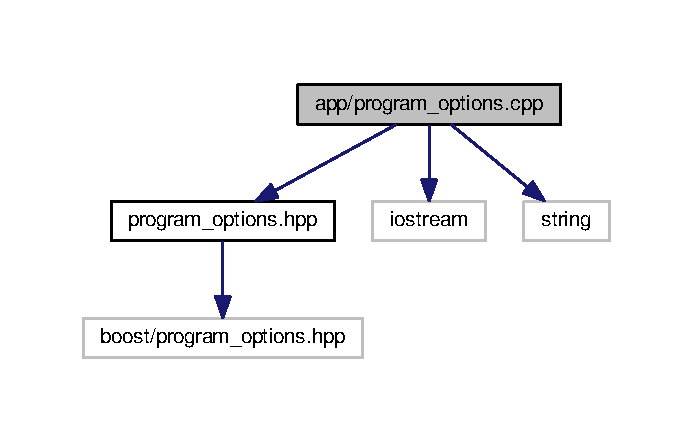
\includegraphics[width=333pt]{program__options_8cpp__incl}
\end{center}
\end{figure}


\subsection{Detailed Description}
This class allows for command line arguments for file paths. 

\begin{DoxyAuthor}{Author}
Pablo Sanhueza 

Ryan Cunningham 

Andre Gomes 
\end{DoxyAuthor}
\begin{DoxyCopyright}{Copyright}
2019 Pablo Sanhueza, Ryan Cunningham, Andre Gomes Distributed under the B\+SD License (license terms found in L\+I\+C\+E\+N\+SE or at \href{https://www.freebsd.org/copyright/freebsd-license.html}{\tt https\+://www.\+freebsd.\+org/copyright/freebsd-\/license.\+html}) 
\end{DoxyCopyright}

\hypertarget{data_8hpp}{}\section{include/data.hpp File Reference}
\label{data_8hpp}\index{include/data.\+hpp@{include/data.\+hpp}}


Loads data files (images).  


{\ttfamily \#include $<$opencv2/opencv.\+hpp$>$}\\*
{\ttfamily \#include $<$string$>$}\\*
{\ttfamily \#include $<$vector$>$}\\*
Include dependency graph for data.\+hpp\+:
\nopagebreak
\begin{figure}[H]
\begin{center}
\leavevmode
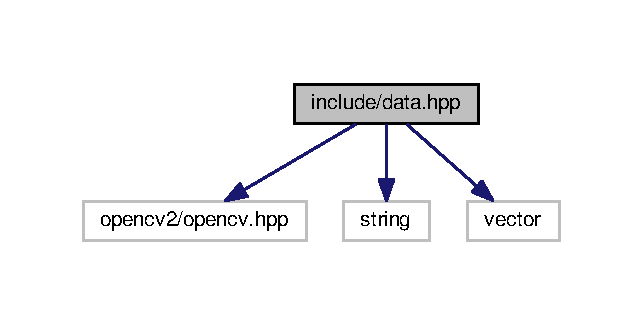
\includegraphics[width=309pt]{data_8hpp__incl}
\end{center}
\end{figure}
This graph shows which files directly or indirectly include this file\+:
\nopagebreak
\begin{figure}[H]
\begin{center}
\leavevmode
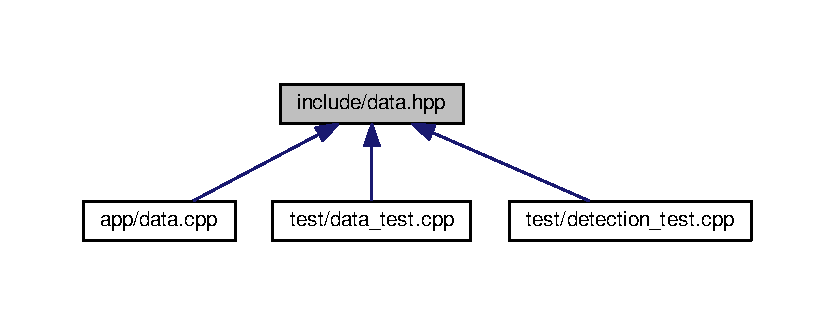
\includegraphics[width=350pt]{data_8hpp__dep__incl}
\end{center}
\end{figure}
\subsection*{Classes}
\begin{DoxyCompactItemize}
\item 
class \hyperlink{classData}{Data}
\end{DoxyCompactItemize}


\subsection{Detailed Description}
Loads data files (images). 

\begin{DoxyAuthor}{Author}
Pablo Sanhueza 

Ryan Cunningham 

Andre Gomes 
\end{DoxyAuthor}
\begin{DoxyCopyright}{Copyright}
2019 Group16 Distributed under the B\+SD License (license terms found in L\+I\+C\+E\+N\+SE or at \href{https://www.freebsd.org/copyright/freebsd-license.html}{\tt https\+://www.\+freebsd.\+org/copyright/freebsd-\/license.\+html}) 
\end{DoxyCopyright}

\hypertarget{detection_8hpp}{}\section{include/detection.hpp File Reference}
\label{detection_8hpp}\index{include/detection.\+hpp@{include/detection.\+hpp}}
{\ttfamily \#include $<$opencv2/opencv.\+hpp$>$}\\*
{\ttfamily \#include $<$vector$>$}\\*
Include dependency graph for detection.\+hpp\+:
\nopagebreak
\begin{figure}[H]
\begin{center}
\leavevmode
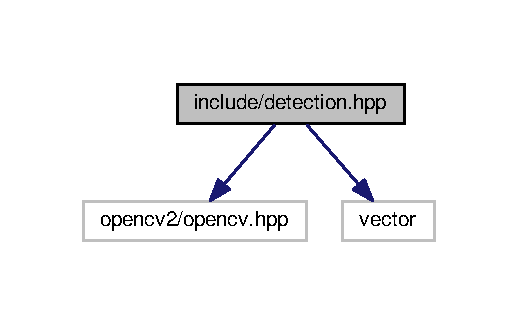
\includegraphics[width=249pt]{detection_8hpp__incl}
\end{center}
\end{figure}
This graph shows which files directly or indirectly include this file\+:
\nopagebreak
\begin{figure}[H]
\begin{center}
\leavevmode
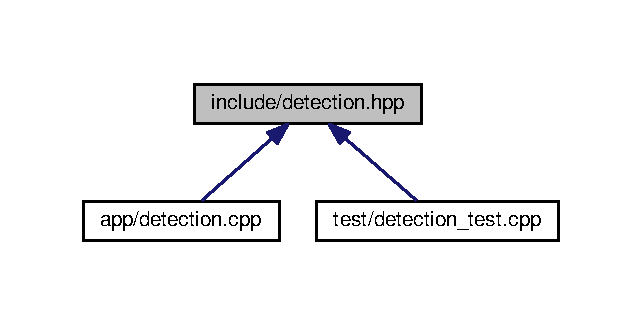
\includegraphics[width=308pt]{detection_8hpp__dep__incl}
\end{center}
\end{figure}
\subsection*{Classes}
\begin{DoxyCompactItemize}
\item 
class \hyperlink{classDetection}{Detection}
\end{DoxyCompactItemize}


\subsection{Detailed Description}
\begin{DoxyAuthor}{Author}

\end{DoxyAuthor}
\begin{DoxyCopyright}{Copyright}
2019 Distributed under the B\+SD License (license terms found in L\+I\+C\+E\+N\+SE or at \href{https://www.freebsd.org/copyright/freebsd-license.html}{\tt https\+://www.\+freebsd.\+org/copyright/freebsd-\/license.\+html}) 
\end{DoxyCopyright}

\hypertarget{locator_8hpp}{}\section{include/locator.hpp File Reference}
\label{locator_8hpp}\index{include/locator.\+hpp@{include/locator.\+hpp}}


End result of class is to return the position of the object desired. Class will receive dimensions and starting pixel position of a bounding box, and from there determine the world coordinate position depending on the camera. Here we assume the intrinsic and extrinsic parameters of the camera.  


{\ttfamily \#include $<$vector$>$}\\*
{\ttfamily \#include $<$opencv2/opencv.\+hpp$>$}\\*
Include dependency graph for locator.\+hpp\+:
\nopagebreak
\begin{figure}[H]
\begin{center}
\leavevmode
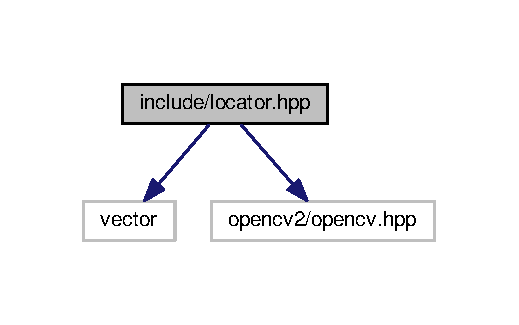
\includegraphics[width=249pt]{locator_8hpp__incl}
\end{center}
\end{figure}
This graph shows which files directly or indirectly include this file\+:
\nopagebreak
\begin{figure}[H]
\begin{center}
\leavevmode
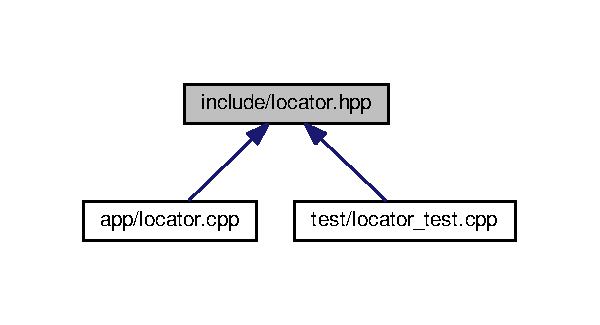
\includegraphics[width=288pt]{locator_8hpp__dep__incl}
\end{center}
\end{figure}
\subsection*{Classes}
\begin{DoxyCompactItemize}
\item 
class \hyperlink{classLocator}{Locator}
\end{DoxyCompactItemize}


\subsection{Detailed Description}
End result of class is to return the position of the object desired. Class will receive dimensions and starting pixel position of a bounding box, and from there determine the world coordinate position depending on the camera. Here we assume the intrinsic and extrinsic parameters of the camera. 

Copyright (C) 2019 -\/ Group16\+: Pablo Sanhueza, Andre Gomes, \& Ryan Cunningham \begin{DoxyAuthor}{Author}
Pablo Sanhueza 

Andre Gomes 

Ryan Cunningham
\end{DoxyAuthor}
\begin{DoxyCopyright}{Copyright}
Copyright 2019 Group16 Distributed under the B\+SD License (license terms found in L\+I\+C\+E\+N\+SE or at \href{https://www.freebsd.org/copyright/freebsd-license.html}{\tt https\+://www.\+freebsd.\+org/copyright/freebsd-\/license.\+html}) 
\end{DoxyCopyright}

\hypertarget{program__options_8hpp}{}\section{include/program\+\_\+options.hpp File Reference}
\label{program__options_8hpp}\index{include/program\+\_\+options.\+hpp@{include/program\+\_\+options.\+hpp}}


Class allows for command line arguments for setting path.  


{\ttfamily \#include $<$boost/program\+\_\+options.\+hpp$>$}\\*
Include dependency graph for program\+\_\+options.\+hpp\+:
\nopagebreak
\begin{figure}[H]
\begin{center}
\leavevmode
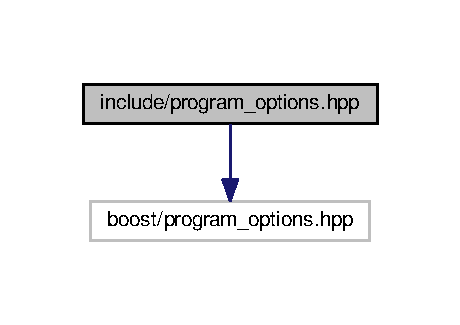
\includegraphics[width=221pt]{program__options_8hpp__incl}
\end{center}
\end{figure}
This graph shows which files directly or indirectly include this file\+:
\nopagebreak
\begin{figure}[H]
\begin{center}
\leavevmode
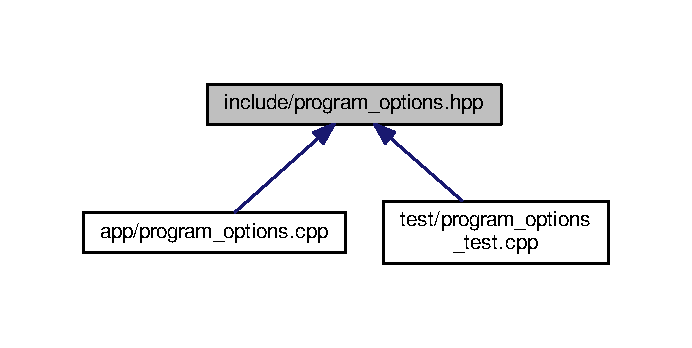
\includegraphics[width=332pt]{program__options_8hpp__dep__incl}
\end{center}
\end{figure}
\subsection*{Classes}
\begin{DoxyCompactItemize}
\item 
class \hyperlink{classProgramOptions}{Program\+Options}
\end{DoxyCompactItemize}


\subsection{Detailed Description}
Class allows for command line arguments for setting path. 

\begin{DoxyAuthor}{Author}
Ryan Cunningham 

Pablo Sanhueza 

Andre Gomes 
\end{DoxyAuthor}
\begin{DoxyCopyright}{Copyright}
2019 Ryan Cunningham, Pablo Sanhueza, Andre Gomes Distributed under the B\+SD License (license terms found in L\+I\+C\+E\+N\+SE or at \href{https://www.freebsd.org/copyright/freebsd-license.html}{\tt https\+://www.\+freebsd.\+org/copyright/freebsd-\/license.\+html}) 
\end{DoxyCopyright}

\hypertarget{data__test_8cpp}{}\section{test/data\+\_\+test.cpp File Reference}
\label{data__test_8cpp}\index{test/data\+\_\+test.\+cpp@{test/data\+\_\+test.\+cpp}}


Unit Test for \hyperlink{classData}{Data} Class.  


{\ttfamily \#include \char`\"{}data.\+hpp\char`\"{}}\\*
{\ttfamily \#include $<$boost/filesystem.\+hpp$>$}\\*
{\ttfamily \#include $<$gtest/gtest.\+h$>$}\\*
{\ttfamily \#include $<$string$>$}\\*
{\ttfamily \#include $<$vector$>$}\\*
Include dependency graph for data\+\_\+test.\+cpp\+:
\nopagebreak
\begin{figure}[H]
\begin{center}
\leavevmode
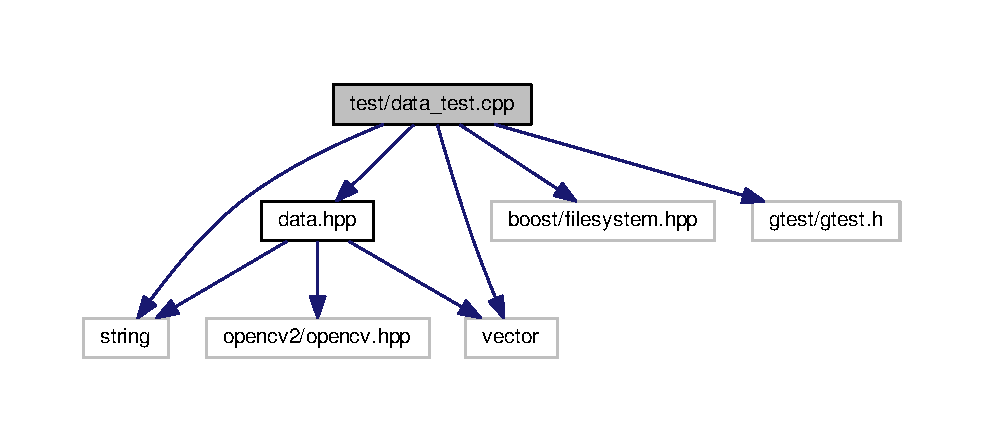
\includegraphics[width=350pt]{data__test_8cpp__incl}
\end{center}
\end{figure}
\subsection*{Functions}
\begin{DoxyCompactItemize}
\item 
{\bfseries T\+E\+ST} (Data\+Test, test\+Load\+Images)\hypertarget{data__test_8cpp_a4ace6ba45da910655d845cd8d9db8d57}{}\label{data__test_8cpp_a4ace6ba45da910655d845cd8d9db8d57}

\end{DoxyCompactItemize}


\subsection{Detailed Description}
Unit Test for \hyperlink{classData}{Data} Class. 

\begin{DoxyAuthor}{Author}
Pablo Sanhueza 

Ryan Cunningham 

Andre Gomes 
\end{DoxyAuthor}
\begin{DoxyCopyright}{Copyright}
2019 Pablo Sanhuez, Ryan Cunningham, Andre Gomes Distributed under the B\+SD License (license terms found in L\+I\+C\+E\+N\+SE or at \href{https://www.freebsd.org/copyright/freebsd-license.html}{\tt https\+://www.\+freebsd.\+org/copyright/freebsd-\/license.\+html}) 
\end{DoxyCopyright}

\hypertarget{detection__test_8cpp}{}\section{test/detection\+\_\+test.cpp File Reference}
\label{detection__test_8cpp}\index{test/detection\+\_\+test.\+cpp@{test/detection\+\_\+test.\+cpp}}


Unit Test for \hyperlink{classDetection}{Detection} Class.  


{\ttfamily \#include \char`\"{}detection.\+hpp\char`\"{}}\\*
{\ttfamily \#include $<$gtest/gtest.\+h$>$}\\*
{\ttfamily \#include $<$opencv2/opencv.\+hpp$>$}\\*
{\ttfamily \#include $<$string$>$}\\*
{\ttfamily \#include $<$vector$>$}\\*
{\ttfamily \#include \char`\"{}data.\+hpp\char`\"{}}\\*
Include dependency graph for detection\+\_\+test.\+cpp\+:
\nopagebreak
\begin{figure}[H]
\begin{center}
\leavevmode
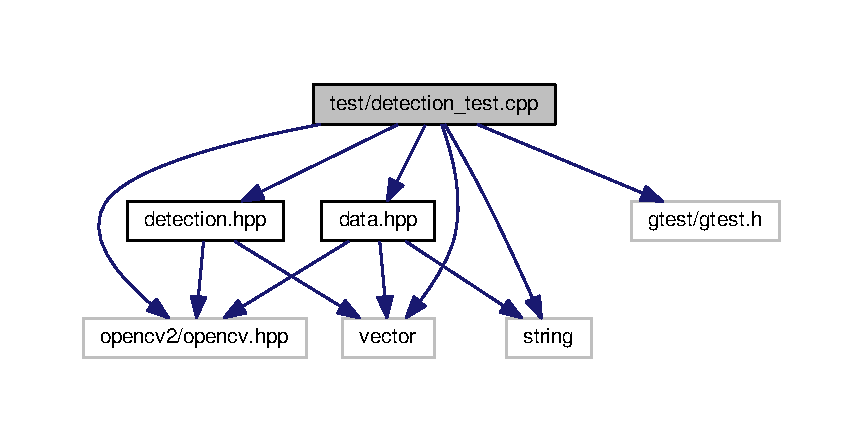
\includegraphics[width=350pt]{detection__test_8cpp__incl}
\end{center}
\end{figure}
\subsection*{Functions}
\begin{DoxyCompactItemize}
\item 
{\bfseries T\+E\+ST} (Detection\+Test, test\+No\+Human\+In\+Image)\hypertarget{detection__test_8cpp_a9dbcf305e237eafe62f4a3506d76e442}{}\label{detection__test_8cpp_a9dbcf305e237eafe62f4a3506d76e442}

\item 
{\bfseries T\+E\+ST} (Detection\+Test, test\+Human\+In\+Image)\hypertarget{detection__test_8cpp_a2b010bc43233d0269cf29b85fd24fb6f}{}\label{detection__test_8cpp_a2b010bc43233d0269cf29b85fd24fb6f}

\item 
{\bfseries T\+E\+ST} (Detection\+Test, test\+Mulitple\+Humans\+In\+Image)\hypertarget{detection__test_8cpp_a59348bd0970b092451538b93d3847768}{}\label{detection__test_8cpp_a59348bd0970b092451538b93d3847768}

\end{DoxyCompactItemize}


\subsection{Detailed Description}
Unit Test for \hyperlink{classDetection}{Detection} Class. 

\begin{DoxyAuthor}{Author}
Andre Gomes 

Pablo Sanhueza 

Ryan Cunningham 
\end{DoxyAuthor}
\begin{DoxyCopyright}{Copyright}
2019 Andre Gomes, Pablo Sanhueza, Ryan Cunningham Distributed under the B\+SD License (license terms found in L\+I\+C\+E\+N\+SE or at \href{https://www.freebsd.org/copyright/freebsd-license.html}{\tt https\+://www.\+freebsd.\+org/copyright/freebsd-\/license.\+html}) 
\end{DoxyCopyright}

\hypertarget{locator__test_8cpp}{}\section{test/locator\+\_\+test.cpp File Reference}
\label{locator__test_8cpp}\index{test/locator\+\_\+test.\+cpp@{test/locator\+\_\+test.\+cpp}}


Unit Tests for \hyperlink{classLocator}{Locator}.  


{\ttfamily \#include $<$gtest/gtest.\+h$>$}\\*
{\ttfamily \#include $<$opencv2/opencv.\+hpp$>$}\\*
{\ttfamily \#include $<$vector$>$}\\*
{\ttfamily \#include \char`\"{}locator.\+hpp\char`\"{}}\\*
Include dependency graph for locator\+\_\+test.\+cpp\+:
\nopagebreak
\begin{figure}[H]
\begin{center}
\leavevmode
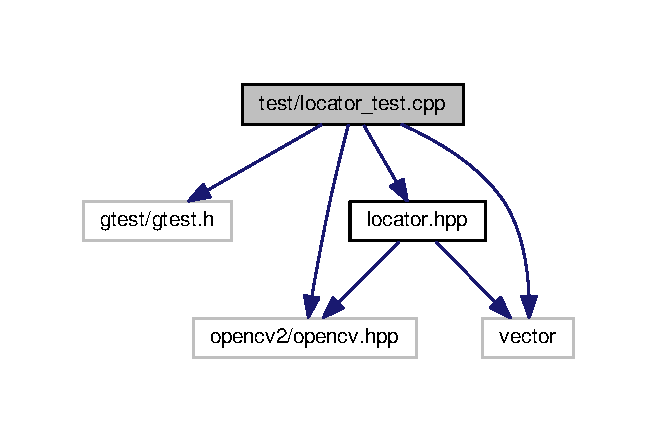
\includegraphics[width=316pt]{locator__test_8cpp__incl}
\end{center}
\end{figure}
\subsection*{Functions}
\begin{DoxyCompactItemize}
\item 
\hyperlink{locator__test_8cpp_a220b42f605fa9dedb81bc399fadf3b2c}{T\+E\+ST} (Locator\+Test, test\+Default\+Locator)
\item 
\hyperlink{locator__test_8cpp_a6b5222818ca559c9a3348c1c0eb32e69}{T\+E\+ST} (Locator\+Test, test\+Locator\+Constructor)
\item 
\hyperlink{locator__test_8cpp_a9aff7c95f2920240392f1b87474a737c}{T\+E\+ST} (Locator\+Test, test\+Set\+Pixel\+Data)
\item 
\hyperlink{locator__test_8cpp_a7b2120d471025b66b53503f096df1bc2}{T\+E\+ST} (Locator\+Test, test\+World\+Pos)
\end{DoxyCompactItemize}


\subsection{Detailed Description}
Unit Tests for \hyperlink{classLocator}{Locator}. 

\begin{DoxyAuthor}{Author}
Pablo Sanhueza 

Ryan Cunningham 

Andre Gomes
\end{DoxyAuthor}
\begin{DoxyCopyright}{Copyright}
2019 
\end{DoxyCopyright}


\subsection{Function Documentation}
\index{locator\+\_\+test.\+cpp@{locator\+\_\+test.\+cpp}!T\+E\+ST@{T\+E\+ST}}
\index{T\+E\+ST@{T\+E\+ST}!locator\+\_\+test.\+cpp@{locator\+\_\+test.\+cpp}}
\subsubsection[{\texorpdfstring{T\+E\+S\+T(\+Locator\+Test, test\+Default\+Locator)}{TEST(LocatorTest, testDefaultLocator)}}]{\setlength{\rightskip}{0pt plus 5cm}T\+E\+ST (
\begin{DoxyParamCaption}
\item[{Locator\+Test}]{, }
\item[{test\+Default\+Locator}]{}
\end{DoxyParamCaption}
)}\hypertarget{locator__test_8cpp_a220b42f605fa9dedb81bc399fadf3b2c}{}\label{locator__test_8cpp_a220b42f605fa9dedb81bc399fadf3b2c}
Tests Default Constructor. Create locator object

Test values to ensure default constructor is initialized to correct values.

Boolean check to determine if test can pass. This is used since it E\+X\+P\+E\+C\+T\+\_\+\+E\+Q() doesn\textquotesingle{}t like dealing with cv\+::\+Mat. \index{locator\+\_\+test.\+cpp@{locator\+\_\+test.\+cpp}!T\+E\+ST@{T\+E\+ST}}
\index{T\+E\+ST@{T\+E\+ST}!locator\+\_\+test.\+cpp@{locator\+\_\+test.\+cpp}}
\subsubsection[{\texorpdfstring{T\+E\+S\+T(\+Locator\+Test, test\+Locator\+Constructor)}{TEST(LocatorTest, testLocatorConstructor)}}]{\setlength{\rightskip}{0pt plus 5cm}T\+E\+ST (
\begin{DoxyParamCaption}
\item[{Locator\+Test}]{, }
\item[{test\+Locator\+Constructor}]{}
\end{DoxyParamCaption}
)}\hypertarget{locator__test_8cpp_a6b5222818ca559c9a3348c1c0eb32e69}{}\label{locator__test_8cpp_a6b5222818ca559c9a3348c1c0eb32e69}
Test Constructor. Create locator object

Test values to ensure default constructor is initialized to correct values.

Boolean check to determine if test can pass. This is used since it E\+X\+P\+E\+C\+T\+\_\+\+E\+Q() doesn\textquotesingle{}t like dealing with cv\+::\+Mat. \index{locator\+\_\+test.\+cpp@{locator\+\_\+test.\+cpp}!T\+E\+ST@{T\+E\+ST}}
\index{T\+E\+ST@{T\+E\+ST}!locator\+\_\+test.\+cpp@{locator\+\_\+test.\+cpp}}
\subsubsection[{\texorpdfstring{T\+E\+S\+T(\+Locator\+Test, test\+Set\+Pixel\+Data)}{TEST(LocatorTest, testSetPixelData)}}]{\setlength{\rightskip}{0pt plus 5cm}T\+E\+ST (
\begin{DoxyParamCaption}
\item[{Locator\+Test}]{, }
\item[{test\+Set\+Pixel\+Data}]{}
\end{DoxyParamCaption}
)}\hypertarget{locator__test_8cpp_a9aff7c95f2920240392f1b87474a737c}{}\label{locator__test_8cpp_a9aff7c95f2920240392f1b87474a737c}
Tests set\+Pixel\+Data() method from \hyperlink{classLocator}{Locator} Class. Create locator object

Valid arguments to create rectangle

Create rectangle...

Sets pixel data for testing \index{locator\+\_\+test.\+cpp@{locator\+\_\+test.\+cpp}!T\+E\+ST@{T\+E\+ST}}
\index{T\+E\+ST@{T\+E\+ST}!locator\+\_\+test.\+cpp@{locator\+\_\+test.\+cpp}}
\subsubsection[{\texorpdfstring{T\+E\+S\+T(\+Locator\+Test, test\+World\+Pos)}{TEST(LocatorTest, testWorldPos)}}]{\setlength{\rightskip}{0pt plus 5cm}T\+E\+ST (
\begin{DoxyParamCaption}
\item[{Locator\+Test}]{, }
\item[{test\+World\+Pos}]{}
\end{DoxyParamCaption}
)}\hypertarget{locator__test_8cpp_a7b2120d471025b66b53503f096df1bc2}{}\label{locator__test_8cpp_a7b2120d471025b66b53503f096df1bc2}
Tests world\+Pos() method from \hyperlink{classLocator}{Locator} Class. Create locator object

Valid arguments to create rectangle

Create rectangle...

Test Coordinate results computed by beforehand using formula -\/$>$ \mbox{[}X, Y, Z\mbox{]} = ((\mbox{[}u, v, 1\mbox{]} $\ast$ Intrin\+\_\+\+Matrix\+\_\+\+Inv) -\/ \mbox{[}tx, ty, tz\mbox{]} ) $\ast$ Rot\+\_\+\+Matrix\+\_\+\+Inv

Sets pixel data for testing

Takes difference of all elements in matrix and compares them

Boolean check to determine if test can pass. This is used since it E\+X\+P\+E\+C\+T\+\_\+\+E\+Q() doesn\textquotesingle{}t like dealing with cv\+::\+Mat. 
\hypertarget{program__options__test_8cpp}{}\section{test/program\+\_\+options\+\_\+test.cpp File Reference}
\label{program__options__test_8cpp}\index{test/program\+\_\+options\+\_\+test.\+cpp@{test/program\+\_\+options\+\_\+test.\+cpp}}


Unit Test for \hyperlink{classProgramOptions}{Program\+Options} Class.  


{\ttfamily \#include \char`\"{}program\+\_\+options.\+hpp\char`\"{}}\\*
{\ttfamily \#include $<$gtest/gtest.\+h$>$}\\*
{\ttfamily \#include $<$string$>$}\\*
{\ttfamily \#include $<$vector$>$}\\*
Include dependency graph for program\+\_\+options\+\_\+test.\+cpp\+:
\nopagebreak
\begin{figure}[H]
\begin{center}
\leavevmode
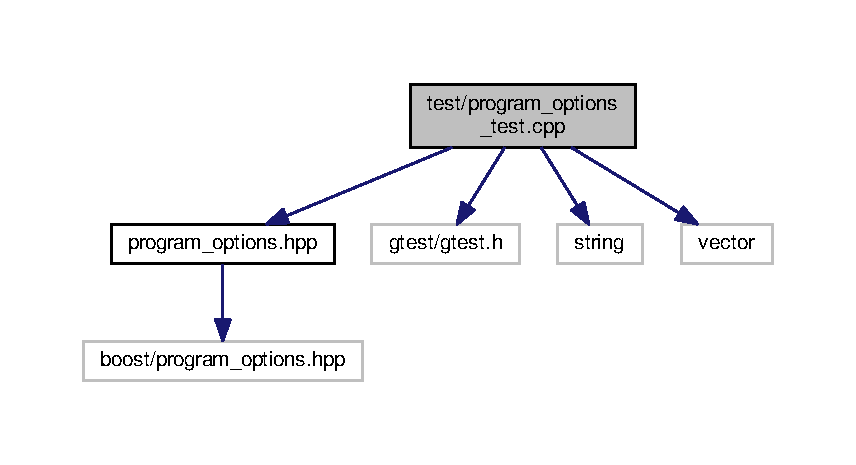
\includegraphics[width=350pt]{program__options__test_8cpp__incl}
\end{center}
\end{figure}
\subsection*{Functions}
\begin{DoxyCompactItemize}
\item 
{\bfseries T\+E\+ST} (Program\+Options\+Test, test\+No\+Options)\hypertarget{program__options__test_8cpp_ae4a3fb6f064471c7c2ed23d73a3f8b68}{}\label{program__options__test_8cpp_ae4a3fb6f064471c7c2ed23d73a3f8b68}

\item 
{\bfseries T\+E\+ST} (Program\+Options\+Test, test\+Get\+Value\+Not\+Provided)\hypertarget{program__options__test_8cpp_a7eee0e5675f6f7c2475d0da47fe13c6c}{}\label{program__options__test_8cpp_a7eee0e5675f6f7c2475d0da47fe13c6c}

\item 
{\bfseries T\+E\+ST} (Program\+Options\+Test, test\+Get\+Value\+Provided)\hypertarget{program__options__test_8cpp_aedbd839fdaaa2620c8e9ebed2599539a}{}\label{program__options__test_8cpp_aedbd839fdaaa2620c8e9ebed2599539a}

\end{DoxyCompactItemize}


\subsection{Detailed Description}
Unit Test for \hyperlink{classProgramOptions}{Program\+Options} Class. 

\begin{DoxyAuthor}{Author}
Andre Gomes 

Pablo Sanhueza 

Ryan Cunningham 
\end{DoxyAuthor}
\begin{DoxyCopyright}{Copyright}
2019 Andre Gomes, Pablo Sanhueza, Ryan Cunningham Distributed under the B\+SD License (license terms found in L\+I\+C\+E\+N\+SE or at \href{https://www.freebsd.org/copyright/freebsd-license.html}{\tt https\+://www.\+freebsd.\+org/copyright/freebsd-\/license.\+html}) 
\end{DoxyCopyright}

%--- End generated contents ---

% Index
\backmatter
\newpage
\phantomsection
\clearemptydoublepage
\addcontentsline{toc}{chapter}{Index}
\printindex

\end{document}
